% !TEX program = xelatex
% =====================================================================
%  slides.tex  --  example deck for the mynotes Beamer theme.
%  Copy this file to start a new talk. Every component of the notes
%  (boxes, callouts, code, tables, figures) works here the same way.
% =====================================================================
\documentclass[aspectratio=169, 9pt, t, notheorems]{beamer}
%   aspectratio=169 : widescreen (use 43 for 4:3 projectors)
%   9pt             : more content per slide (10pt / 11pt for bigger text)
%   t               : content starts at the top of each slide
%   notheorems      : required, so the template's boxes replace Beamer's theorems
\usetheme{mynotes}          % [sectionframes] adds a slide at every \section,
                            % [nonavigation] hides the navigation bar at the top

\title[Short Title]{Presentation Title}   % [short title] appears in the footer
\subtitle{An optional subtitle for the talk}
\author{Author Name}
\website{https://example.com}              % the author name links here
\institute{Department Name, University Name}
\date{\today}

\begin{document}

\titleframe   % title slide (no header or footer)

% ---------------------------------------------------------------------
\begin{frame}{Outline}
  \tableofcontents
\end{frame}

% =====================================================================
\section{Introduction}     % section names appear in the navigation bar
% =====================================================================

\begin{frame}{Text and lists}{Frame titles can have a subtitle}
  Slides use the same typeface and colors as the notes, with
  \hl{highlighting}, \alert{alerts} and \emph{emphasis}.
  \begin{itemize}
    \item a first point
    \item a second point
    \begin{itemize}
      \item sub-points get a dash
    \end{itemize}
    \item a third point
  \end{itemize}
  \begin{enumerate}
    \item a numbered step
    \item another step
    \item the last step
  \end{enumerate}
  % Reveal content step by step with \pause, or with \item<2-> etc.
\end{frame}

\begin{frame}{Two columns}
  \begin{columns}[T]
    \begin{column}{0.48\textwidth}
      \begin{definition}[Title][def:sample]
        A definition box with a title and a label:
        \[ p(x) = \sum_{k=0}^{n} a_k x^k \]
      \end{definition}
      Text continues below the box, in the same column.
    \end{column}
    \begin{column}{0.48\textwidth}
      \centering
      \begin{tikzpicture}[>=Stealth, thick, font=\small, node distance=0.7cm,
          box/.style={draw=accent, fill=accent!8, rounded corners=4pt,
                      inner sep=6pt, minimum width=1.5cm}]
        \node[box] (in) {Input};
        \node[box, right=of in] (proc) {Process};
        \node[box, right=of proc] (out) {Output};
        \draw[->] (in) -- (proc);
        \draw[->] (proc) -- (out);
        \draw[->] (out.south) -- ++(0,-0.6) -| node[pos=0.25, below]{feedback}
          (proc.south);
      \end{tikzpicture}
    \end{column}
  \end{columns}
\end{frame}

% =====================================================================
\section{Content}
% =====================================================================

\begin{frame}{Numbered boxes}
  \begin{theorem}[Title of the theorem][thm:sample]
    Statement of the theorem. For all $a, b \ge 0$,
    \[ \frac{a + b}{2} \ge \sqrt{ab}. \]
  \end{theorem}
  \begin{proof}
    Expand $\bigl(\sqrt{a} - \sqrt{b}\bigr)^2 \ge 0$; see also \cref{def:sample}.
  \end{proof}
  \begin{example}
    For $a = 1$ and $b = 4$: $\frac{1 + 4}{2} = 2.5 \ge 2 = \sqrt{4}$.
  \end{example}
  \begin{remark}
    On slides, box titles run into the text to save space.
  \end{remark}
\end{frame}

\begin{frame}{Callouts}
  \begin{columns}[T]
    \begin{column}{0.48\textwidth}
      \begin{tip}[A custom title]
        Any callout accepts a custom title.
      \end{tip}
      \begin{warning}
        A common mistake or a condition that must hold.
      \end{warning}
      \begin{info}
        Background information or a quick fact.
      \end{info}
    \end{column}
    \begin{column}{0.48\textwidth}
      \begin{question}
        A question for the audience.
      \end{question}
      \begin{success}
        A confirmed result.
      \end{success}
      \begin{danger}
        A step that can cause serious errors.
      \end{danger}
    \end{column}
  \end{columns}
\end{frame}

% =====================================================================
\section{Code and data}
% =====================================================================

% Frames with code blocks MUST have [fragile]
\begin{frame}[fragile]{Code}
  \begin{columns}[T]
    \begin{column}{0.56\textwidth}
\begin{python}[example.py]
def mean(values):
    """Arithmetic mean of a list."""
    return sum(values) / len(values)

data = [2, 4, 4, 4, 5, 5, 7, 9]
print(f"mean = {mean(data):.2f}")
\end{python}
    \end{column}
    \begin{column}{0.40\textwidth}
\begin{terminal}
$ python example.py
mean = 5.00
\end{terminal}
      Inline code works too: \code{mean(data)}.
    \end{column}
  \end{columns}
\end{frame}

\begin{frame}{Tables and plots}
  \begin{columns}[c]
    \begin{column}{0.42\textwidth}
      \begin{datatable}[A striped table][tab:sample]{lcr}
        \thead{Item} & \thead{Group} & \thead{Value} \\
        \midrule
        Alpha & A & 12.5 \\
        Beta  & A &  8.0 \\
        Gamma & B & 15.2 \\
        Delta & B &  4.7
      \end{datatable}
    \end{column}
    \begin{column}{0.54\textwidth}
      \begin{notefigure}[A plot drawn with pgfplots][fig:plot]
        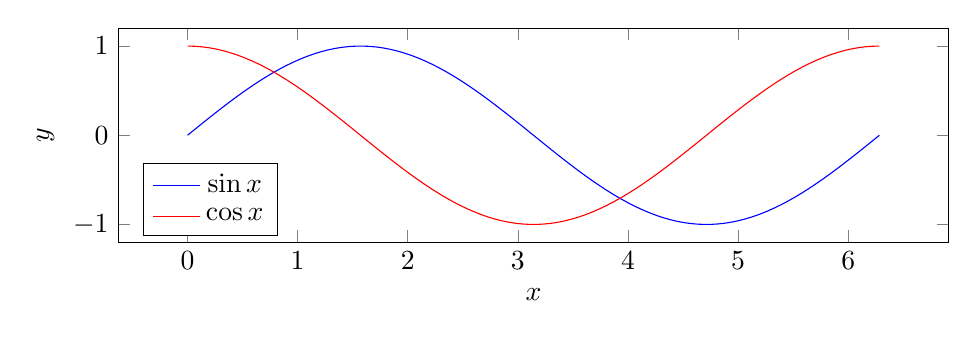
\begin{tikzpicture}
          \begin{axis}[width=\linewidth, height=4.3cm, xlabel={$x$}, ylabel={$y$},
                       domain=0:6.283, samples=100, legend pos=south west]
            \addplot+[no marks] {sin(deg(x))};
            \addplot+[no marks] {cos(deg(x))};
            \legend{$\sin x$, $\cos x$}
          \end{axis}
        \end{tikzpicture}
      \end{notefigure}
    \end{column}
  \end{columns}
\end{frame}

\begin{frame}{Images and pseudocode}
  \begin{columns}[T]
    \begin{column}{0.4\textwidth}
      \begin{notefigure}[An image from a file][fig:image]
        \includegraphics[width=0.8\linewidth]{example-image-a}
      \end{notefigure}
    \end{column}
    \begin{column}{0.56\textwidth}
      \begin{algorithm}[H]
        \caption{A generic iterative procedure}
        \begin{algorithmic}[1]
          \Require data $D$, tolerance $\varepsilon > 0$
          \State $r \gets$ initial guess
          \Repeat
            \For{each item $d \in D$}
              \State update $r$ using $d$
            \EndFor
          \Until{the change in $r$ is below $\varepsilon$}
          \State \Return $r$
        \end{algorithmic}
      \end{algorithm}
    \end{column}
  \end{columns}
\end{frame}

\begin{frame}{Beamer blocks}
  \begin{block}{Block}
    Standard Beamer blocks are restyled to match the theme.
  \end{block}
  \begin{alertblock}{Alert block}
    For something the audience must not miss.
  \end{alertblock}
  \begin{exampleblock}{Example block}
    Cross-references work as in the notes: \cref{thm:sample}, \cref{tab:sample}
    and \cref{fig:plot}.
  \end{exampleblock}
\end{frame}

% =====================================================================
\section{Summary}
% =====================================================================

\begin{frame}{Summary}
  \begin{summary}
    One style for notes and slides: write once, reuse everywhere.
  \end{summary}
  \begin{itemize}
    \item boxes and callouts look the same as in the notes
    \item code, tables, plots and figures fit on one slide
    \item a navigation bar at the top, slide numbers in the footer
  \end{itemize}
\end{frame}

\closingframe   % "Thank you!" + "Questions & Discussion" (no header or footer)

\end{document}
